% !TEX root=/home/tavant/these/manuscript/src/manuscript.tex

\section{Effect of electron emission}
  \label{sec-see}
  
  In \Cref{sec-canonical}, the walls are not emissive.
  However, the dielectric ceramic used in \ac{HET} can emit electrons \citep{villemant2018,barral2003a}.
  The electron emission model used, introduced in \cref{sec-modelused}, has three parameters $\proba_0, \crover, \probamax$, such that the emission probability depends on the kinetic energy of the incident electron $\ek$ as
  \begin{equation} \label{eq-barral_second}
    \proba = \min \lp \proba_0 + (1 -  \proba_0) \frac{\ek}{\crover}, \probamax    \rp.
  \end{equation}
  
  The value of parameters are summarized in \cref{tab-tabe_parameters_see}.
  The crossover energy $\crover$ is varied from as low as 4~V, corresponding to a very emissive material, to as high as 200~V, a less emissive material.
  
  \begin{table}[hbtp]
  \ra{1.3}
    \centering
    \caption{Parameters of the electron emission probability model}
    \label{tab-tabe_parameters_see}
    \begin{tabular}{@{}ll@{}} \toprule
    Parameter & value  \\ \midrule
    $\proba_0$ & 0.5  \\
    $\probamax$ & 2.9 \\
    $\crover$   &  4  -- 200 V\\
    \bottomrule
    \end{tabular}
  \end{table}
  
  \begin{figure}[hbtp]
    \centering
    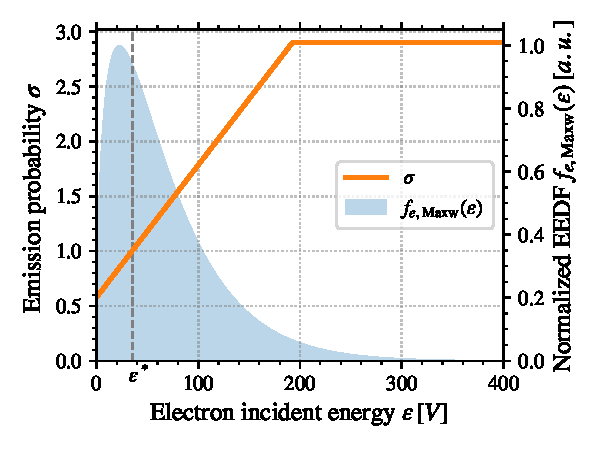
\includegraphics[width=\defaultwidth]{SEE_models}
    \caption{Illustration of the electron emission model of \cref{eq-barral_second} compared to a Maxwellian energy distribution function of temperature of 45~V, with $\crover=35.04$~V.}
    \label{fig-see_illustration}
  \end{figure}
  
  \Cref{fig-see_illustration} shows the electron emission probability for $\crover=35.04$~V compared to a Maxwellian \ac{EEDF} of temperature of 45~V.
  We can see that the saturation of $\proba$ at $\probamax$ happens only for the very high energy tail.
  In the simulation, we can only measure the average electron emission yield, also named emission rate, 
  \begin{equation} \label{eq-seeyield}
    \rate = \frac{\Gamma_{\rm emitted}}{\Gamma_{\rm incident}} = \frac{\iiint v_r \proba(\vect{v}) f(\vect{v}) d^3v}{\iiint v_r  f(\vect{v}) d^3v}.
  \end{equation}
  In general, \cref{eq-seeyield} cannot be calculated analytically.
  However, if we suppose that the \ac{EEDF} is Maxwellian and neglect the saturation at $\probamax$, \cref{eq-seeyield} yields
  \begin{equation} \label{eq-seemaxw}
    \ratemaxw(\Te) = \proba_0 + (1 - \proba_0) \frac{2 \Te}{\crover}.
  \end{equation}
  The saturation at $\probamax$ can be neglected as we have seen that it only affects a small part of the electron population, see \cref{fig-see_illustration}.
  \inlinenote{Add the exact calculation and the relative error ? \\Anne: oui. si trop long, a mettre en annexe.}
  
  \subsection{Impact of the electron emission of the mobility} \label{subsec-param-mob}
    
  The effects of the electron emission at the wall on the electron axial mobility are presented in \Cref{fig-mob-epsstar}.
  The measured mobility $\mobpic$ are shown, as well as the effective mobility $\mobeff$, the saturation estimate $\mobeffsat$ and the classical mobility $\mobcla$, defined in \cref{sec-transport} respectively by \cref{eq-mudef}, \cref{eq-defmobeff}, \cref{eq-mobeffsat} and \cref{eq-mobclas}.
  The values are averaged in time between $t=5 \mus$ and $t=10\mus$, and in space over the azimuthal and radial directions.
  \inlinenote{Anne: For epsilon=0, we have the values presented in section 2.2 without dielectrics.}
  \begin{figure}[hbtp]
    \centering
    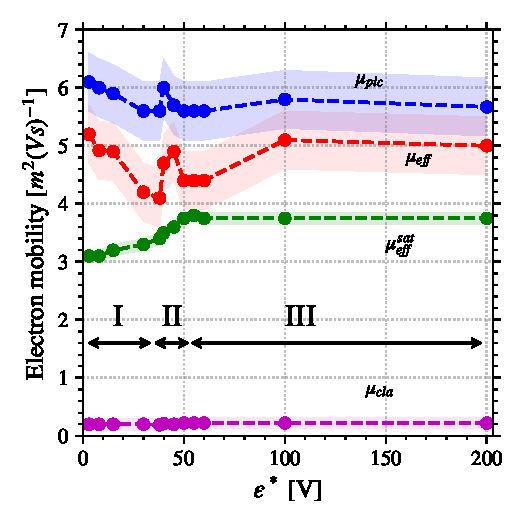
\includegraphics[width=\defaultwidth]{parametric_mobs_eps_complete}
    \caption{Evolution of the electron mobility as a function of the crossover energy $\crover$. In blue $\mobpic$ is the mobility measured in the simulations, while $\mobcla, \mobeff$ and $\mobeffsat$ in purple, red and green respectively are calculated with \cref{eq-mudef,eq-mobclas,eq-defmobeff,eq-mobeffsat}. The three regimes {\bf I, II} and {\bf III}, described in \cref{subsec-regimes} are identified.}
    \label{fig-mob-epsstar}
  \end{figure}
  \inlinenote{Units, in italic !}
  
  As expected, the classical mobility in  \cref{fig-mob-epsstar} is underestimated by more than one order of magnitude compared to $\mobpic$.
  The effective mobility $\mobeff$ and the effective mobility at saturation $\mobeffsat$  are much closer to $\mobpic$, with an underestimation of roughly 10\% and 30\% respectively.
  The mobility measured in the simulation does not evolve much with the electron emission, even for very high emission rate, i.e very low values of $\crover$.
  
  On the other hand, $\mobeffsat$ decreases slightly when $\crover$ decreases from around 40V to lower values.
  However, it still provides a reasonable approximation of the electron enhanced mobility, even with high electron emission rate. 
  
  \subsection{Near wall conductivity}
  
  The results presented in \cref{subsec-param-mob} are spatially averaged.
  However, the mobility coming from the  instability is expected to be higher where the instability is larger, hence at the center of the channel.
  On the other hand, the mobility due to wall emission is located close to the wall \citep{morozov1972}.
  
  \Cref{fig-radial-data} presents the radial profiles of the mobility measured in the \ac{PIC}  simulations without electron emission and for three values of $\crover$.
  On the left, the measured mobility $\mobpic$ is shown and on the right it is the effective mobility $\mobeff$ given by \cref{eq-defmobeff}.
  
  \begin{figure}[hbtp]
    \centering
    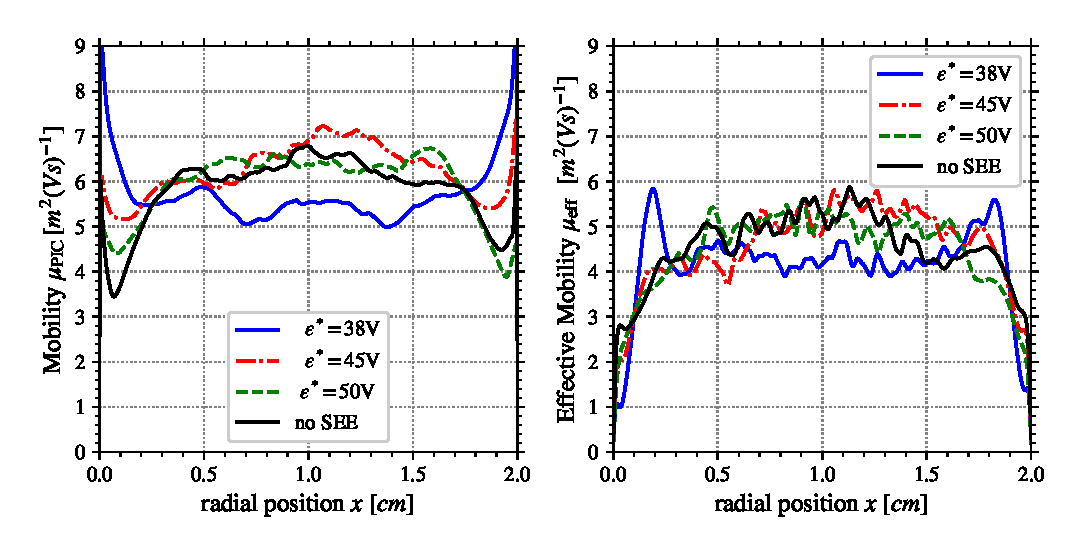
\includegraphics[width=\textwidth]{both_Mobility_SEE}
    \caption{Radial profile the electron mobility (left) measured in the \ac{PIC} simulations, and (right) given by \cref{eq-defmobeff}, for different wall emissivities. }
    \label{fig-radial-data}
  \end{figure}
  
  We can see in \cref{fig-radial-data} that the mobility measured $\mobpic$  in the center decreases by roughly 20\% as the emission rate increases.
  This observation is in agreement with $\mobeffsat$ observed in \cref{fig-radial-data,fig-mob-epsstar}.
  This is due the electron temperature $\Te$ which decreases from around $\Te=45$V at $\crover=200$V to $\Te=30$V at low $\crover$ (the evolution of $\Te$ can be seen in \cref{fig-Tevsproba}).
  
  On the other hand, the near wall mobility increases significantly on $\mobpic$ (almost by a factor of 2) with the increase of the electron emission.
  However, we do not see this evolution on $\mobeffsat$, meaning that it indeed comes from another physical mechanism than the \ac{ECDI}.
  
  
  \subsection{Three different regimes}
  \label{subsec-regimes}

  In \Cref{fig-mob-epsstar}, three regimes have been identified.
  Regime {\bf I} corresponds to low values of $\crover$ (lower than 35V), during which $\mobeffsat$ increases with $\crover$ but $\mobpic$ and $\mobeff$ decreases.
  Regime {\bf III} corresponds to high values of $\crover$ (higher than 50V), during which $\mobeffsat$, and  $\mobpic$ are roughlty constants, but $\mobeff$ increases slightly.
  Regime {\bf II} is a short transition regime, for $35 < \crover < 50$V.
  
  The different regimes are actually obvious when looking at the temporal evolution of the different variables.
  \Cref{fig-threeregimes}  presents the temporal evolution of the space average $\ratepic$ for three different
  values of $\crover$ , corresponding to three different regimes we have identified.
  In regimes {\bf I} and {\bf III}, $\ratepic$ reaches a steady state after a few microseconds.

  \begin{figure}[hbtp]
    \centering
    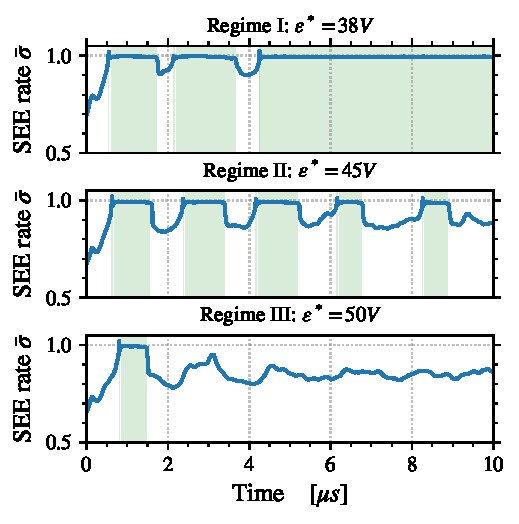
\includegraphics[width=\defaultwidth]{comparaison_3_regimes}
    \caption{Evolution as a function of time of the averaged electron emission rate $\ratepic$ in the three regimes observed (two stables, one with oscillations). The light green zones correspond to the periods when $\ratepic > \ratecr$}
    \label{fig-threeregimes}
  \end{figure}
  

  Regime {\bf I}, with low $\crover$, is characterized by a saturation of $\ratepic$ at a value between $\ratecr$ and 1, which leads to a non-monotonic potential profile.
  Regime {\bf III}, for higher $\crover$, is characterized by a steady state with a SEE rate lower than $\ratecr$.

  The transition between these two stable regimes (monotonic and non-monotonic sheath) passes by regime {\bf II}, an oscillating mode between the two stable regimes.
 As shown in \cref{fig-mob-epsstar}, regime {\bf II} is observed only in a narrow range of $\crover$.
 The oscillations of regime {\bf II} are shown in \cref{fig-threeregimes} up to $10\mus$ but have been observed for more than $40\mus$.
 Note that regimes {\bf I} and {\bf III} in \cref{fig-threeregimes} are obtained for $\crover = 38$~V and $\crover = 50$~V respectively, i.e. near the boundary of the unstable window (see \cref{fig-mob-epsstar}).
 Consequently, we observe a few oscillations before the steady-state is reached, as these cases are close to the bifurcation.
   
   
   The physical origin of the bifurcation can bee seen with the help of \cref{fig-dphivsTe}, which shows the evolution of the potential drop to the wall as a function of the electron temperature.
   It is computed using \cref{eq-seemaxw} for $\rate$ and \cref{eq-sheathhobbs} for the potential drop, which is summarized as 
   \begin{equation} \label{eq-dphi_vs_Te_Maxw}
     \begin{cases}
       \rate = \proba_0 + (1- \proba_0) \frac{2 \Te}{\crover} \\
       \dphi = \Te \ln \lp [1 - \rate] \sqrt{ \frac{m_i}{2 \pi m_e}}  \rp
     \end{cases}
   \end{equation}

   \begin{figure}[hbtp]
     \centering
     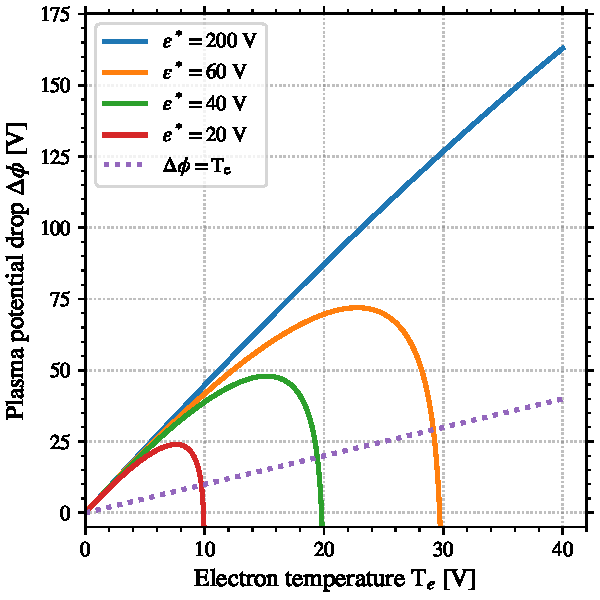
\includegraphics[width=\defaultwidth]{RSO_theo_sheath_bis}
     \caption{Plasma potential drop to the wall as a function of the electron temperature for different values of the cross-over energy $\crover$ using \cref{eq-dphi_vs_Te_Maxw}. The dashed line is $\dphi=\Te$. }
     \label{fig-dphivsTe}
   \end{figure}
   
   \Cref{fig-dphivsTe} shows the evolution of $\dphi$ as a function of $\Te$ obtained with \cref{eq-dphi_vs_Te_Maxw} using four different values of $\crover$. 
   We can see that, starting from low electron temperature, the potential drop increases with the electron temperature, resulting in a better screening of the electrons.
   This corresponds to regime {\bf III}.
   However, the $\dphi$ reaches a maximum, after which it drops sharply to zero and below.
   
   When the potential passes the maximum, the electrons are not screened by the sheath any more.
   Hence, the electrons reach the wall with a higher energy, resulting in a higher electron emission from the wall, hence a smaller potential drop.
   The sheath is unstable, and quickly attains a \ac{SCL} regime \citep{raitses2005}.
   
   In this regime, the sheath is not monotonic, and the model of \cref{eq-sheathhobbs} is no more valid, and the potential drop tends toward $\dphi \simeq \Te$ \citep{hobbs1967,goebel2008} \footnote{see \cref{sec-sheath} for more details}, shown in \cref{fig-dphivsTe}.
   This corresponds to regime {\bf I}.
   
   However, during regime {\bf I}, the electron power losses to the wall are very high, and they can exceed the gains.
   Hence, the electron temperature decreases.
   If $\Te$ decreases too much, the sheath can come back to the previous regime {\bf III}.
   The oscillations between regime {\bf I} and {\bf III} defines regimes {\bf II}.
      
   We have seen in \ref{fig-canon_Te_all} that without electron emission, $\Te$ is of the order of $45$~V.
   Using \cref{fig-dphivsTe}, we can expect to observe the transition between regime {\bf III} and {\bf II} for $\crover \gtrsim 60$~V, as for $\crover = 60$~V, the maximum of $\dphi$ is at $\Te\sim 25$~V, which is significantly lower than 45~V.
   The fact that regime {\bf II} appears at $\crover=50$~V can be explained because
   \begin{enumerate}
     \item a lower $\crover$ increases the electron losses, hence decreases the electron temperature at equilibrium,
     \item the electrons are not Maxwellian.
   \end{enumerate}
   
   The evolution of the temperature with $\crover$ is shown in \cref{fig-Tevsproba}.
   We can see that $\Te \simeq 45\,\volt$ for emission rate up to $\sigma = 0.8$, and decreases down to $\Te=30\,\volt$ for higher emission rates.
   Consequently, even if $\Te$ does indeed decreases when increasing $\crover$, it remains too large compared to the observations of \cref{fig-dphivsTe}.
   The impact of second point will be studied in \cref{ch-3}.
   
   
  